\let\negmedspace\undefined
\let\negthickspace\undefined
\documentclass[journal]{IEEEtran}
\usepackage[a5paper, margin=10mm, onecolumn]{geometry}
\usepackage{lmodern} 
\usepackage{tfrupee} 

\setlength{\headheight}{1cm} 
\setlength{\headsep}{0mm}     

\usepackage{gvv-book}
\usepackage{gvv}
\usepackage{cite}
\usepackage{amsmath,amssymb,amsfonts,amsthm}
\usepackage{algorithmic}
\usepackage{graphicx}
\usepackage{textcomp}
\usepackage{xcolor}
\usepackage{txfonts}
\usepackage{listings}
\usepackage{enumitem}
\usepackage{mathtools}
\usepackage{gensymb}
\usepackage{comment}
\usepackage[breaklinks=true]{hyperref}
\usepackage{tkz-euclide} 

\begin{document}

\bibliographystyle{IEEEtran}

\title{4.7.45}
\author{Revanth Siva Kumar D - EE25BTECH11048
}
{\let\newpage\relax\maketitle}

\textbf{Question} The equation of the line passing through the point $(1, 2)$ and perpendicular to the line $x + y + 1 = 0$ is\\
\textbf{Solution}
Let desired line :
\begin{align}
    \vec{n}^T\vec{x}=c
    \label{eq:question}
\end{align}
Given line equation and point say A:
\begin{align}
    x+y+1=0
    \label{eq:line}\\
    y=-x-1\\
    \vec{A}=\myvec{1\\2}
\end{align}
Since, the line from eq \eqref{eq:line} is perpendicular to \eqref{eq:question} \\
We get the normal vector which is equal to:
\begin{align}
   \vec{n} =\myvec{1\\-1}
\end{align}

Because line \eqref{eq:line} is perpendicular, the equation of the line can be changed as:
\begin{align}
    \vec{n}^T\myvec{\vec{x} - \vec{A}}=0
\end{align}
Thus the equation of line:

\begin{align}
    \myvec{1&-1}\myvec{\vec{x} - \myvec{1\\2}}=0\\
    \implies  \myvec{1&-1}\vec{x}-\myvec{1&-1}\myvec{1\\2}=0\\
    \implies \myvec{1&-1}\vec{x}=-1
\end{align}

\textbf{Final Answer}
The desired line equation is as follows
\begin{align*}
    \myvec{1&-1}\vec{x}=-1
\end{align*}

\begin{figure}
    \centering
    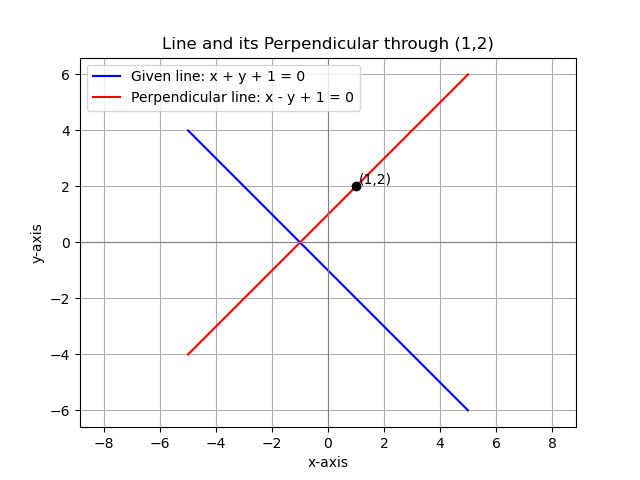
\includegraphics[width=0.8\columnwidth]{figs/Figure_1.png}
    \caption{Plot}
    \label{fig:fig1}
\end{figure}
\end{document}











